\section{Introduction}
\label{sec:intro}

Animals have a variety of ways of communicating information to each other, including vocalizations, behaviors, and smells. 
Among them, vocalizations is one of the most common communication methods for many animals, such as wolves, birds, chimpanzees, and so on. 
Scholars from different fields have been interested in studying vocalizations in animal communication. 
Several studies have demonstrated that vocalizations between animals contain a wealth of information about individuals, behaviors, emotions and contextual environments~\cite{abzaliev2024towards,hantke2018my}.

Human beings can establish a complex communication system through human language and 
use this communication system for information and behavioral interaction. 
Through a structural paradigm, human language can combine phonemes, 
words, sentences to express a variety of complex meanings. 
Previous research has shown that many animals exhibit some of the characteristics in 
human language, albeit to an attenuated version~\citep{kershenbaum2014animal,cartmill2023overcoming}. 
\citet{ficken1994chick}'s work illustrates that Mexican chickadee have simple units of sound and can form a call system with a variety of meanings by combining different units. 
\citet{holland2000coding} illustrates that the call of wren may have an underlying syntactic, elemental structure. 
Bottlenose dolphins show many cognitive and communicative skills that are rare among animals. They are capable not only of generalizing rules, developing abstract concepts and syntactic understanding in an artificial communication system~\citep{janik2000whistle}. 
\citet{gil2000song}'s illustration demonstrates that Phylloscopus trochilus's sound is made up of several recurring elements. 
\citet{favaro2020penguins} has shown that penguin's calls display linguistic similarity with words in human speech.
\citet{leroux2023call}'s work provided evidence for syntactic-like structuring in chimpanzee communication. 
Structured sound sequences produced by humpback whales are described as hierarchically organized songs~\citep{mercado2012understanding}. 
Existing concepts in human language can actually help us to research other animals, as long as we remain critical and open~\citep{meijer2019animal}. 
The study of ``animal language'' can not only reveal more mysteries of the animal world, but also help to explore the origin and evolution of human language~\citep{berthet2023animal}.

The exploration of animal language is a complex and challenge task. One important aspect is 
identifying the basic phonetic units that may exist in animal language. 
Although this is not sufficient to constitute a language, it provides the foundation for exploring the grammatical and meaning information embedded in them. 
Canines are one of the most common domesticated animals, and a large amount of video data can be easily obtained on social media for exploring canine language. 
Recent advancements in machine learning have broadened the path of animal language research, offering the possibility of a data-driven study that can be conducted at a more granular level. Many studies have used machine learning methods to transcribe animal sounds~\citep{huang2023transcribing, hagiwara2024ispa}. 
However this approach is still not completely free from the effects of noise. The presence of noise makes potentially stable structured units more unstable in different environments, thus exacerbating the difficulty of separating the underlying units even further. 
This requires us to design a reliable and interpretable method for discovering candidate basic units in a large number of transcribed texts of high complexity.

\begin{figure*}[th]
	\centering
	\begin{subfigure}[b]{0.3\linewidth}
		\centering
		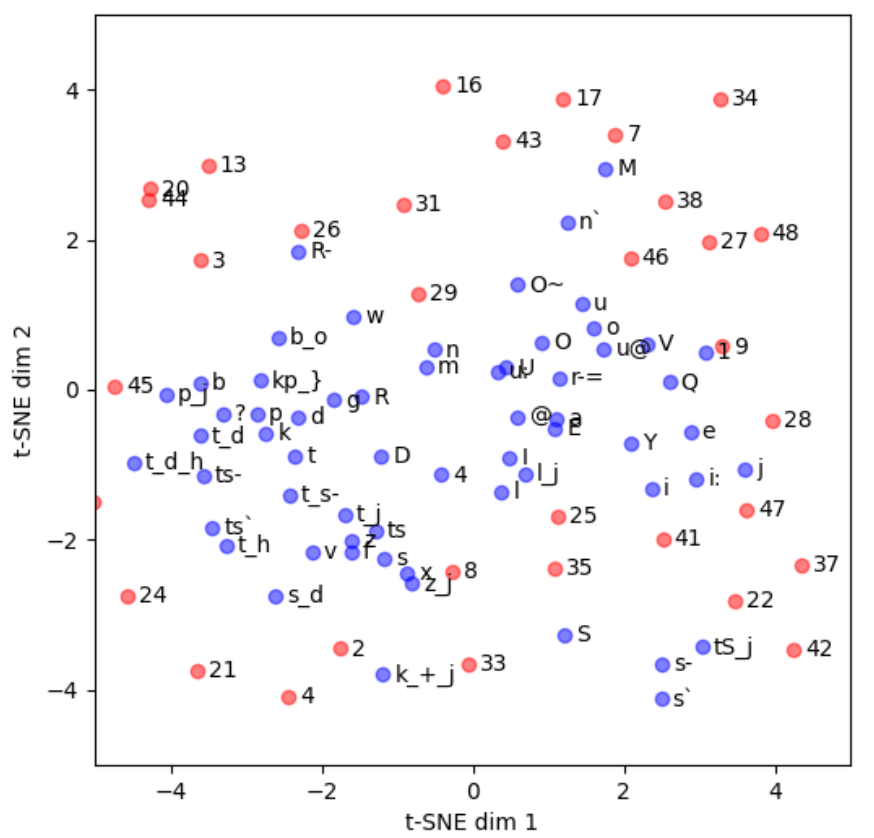
\includegraphics[width=0.95\linewidth]{images/masato.png}
		\caption{2D plot of inter-species phones by \citet{hagiwara2024ispa}.}
		\label{fig:masato}
	\end{subfigure}\quad
	\begin{subfigure}[b]{0.3\linewidth}
		\centering
		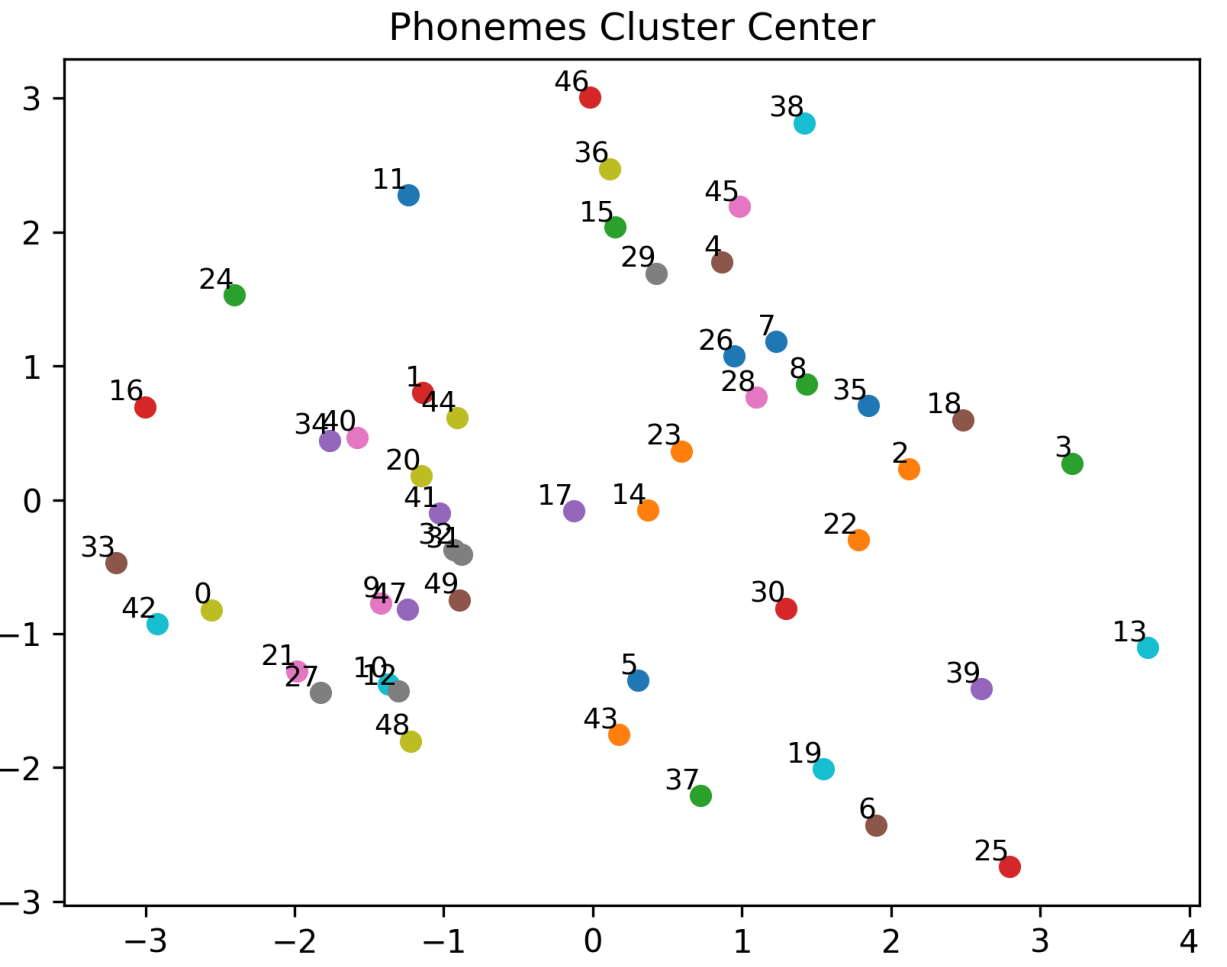
\includegraphics[width=0.95\linewidth]{images/li.png}
		\caption{2D plot of canine phones by \citet{li2024phonetic}.}
		\label{fig:li}
	\end{subfigure}\quad
	\begin{subfigure}[b]{0.3\linewidth}
		\centering
		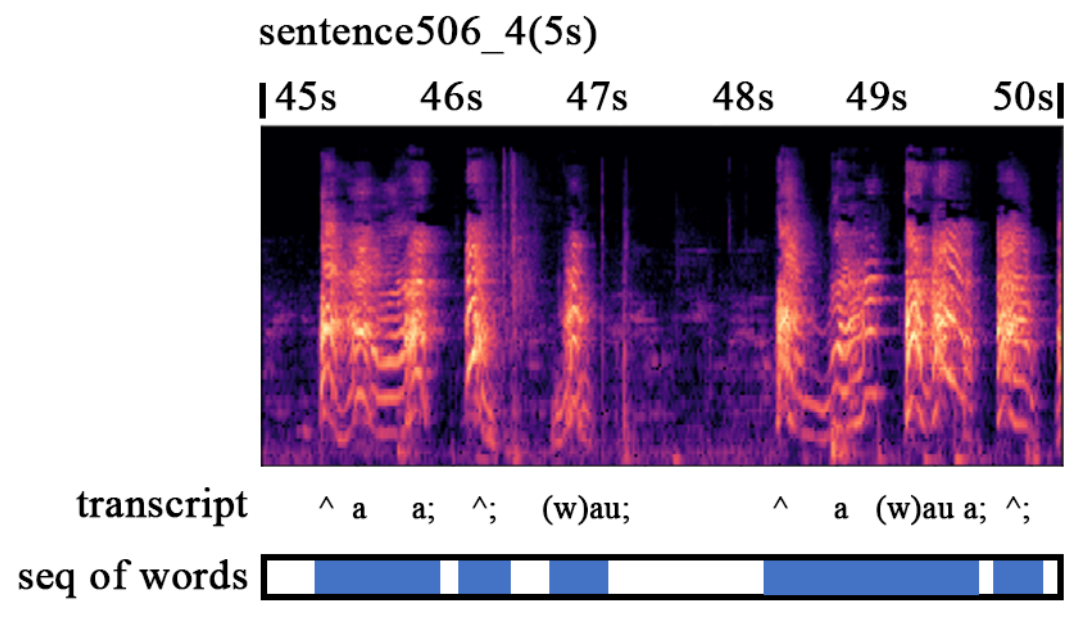
\includegraphics[width=0.95\linewidth]{images/huang.png}
		\caption{A transcript of Shiba Inu~\citep{huang2023transcribing}.}
		\label{fig:huang}
%		\vspace{3cm}
		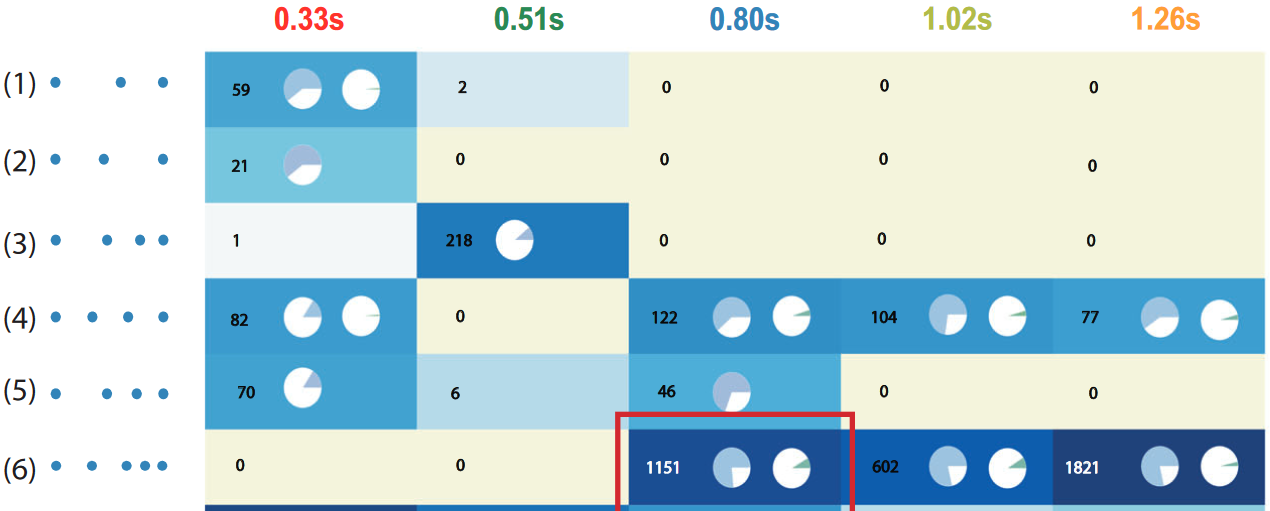
\includegraphics[width=0.95\linewidth]{images/whale.png}
		\caption{Part of sperm whale phonetic alphabet~\citep{sharma2024contextual}.}
		\label{fig:whale}
	\end{subfigure}
%	\begin{subfigure}{0.23\linewidth}
%		\centering
%		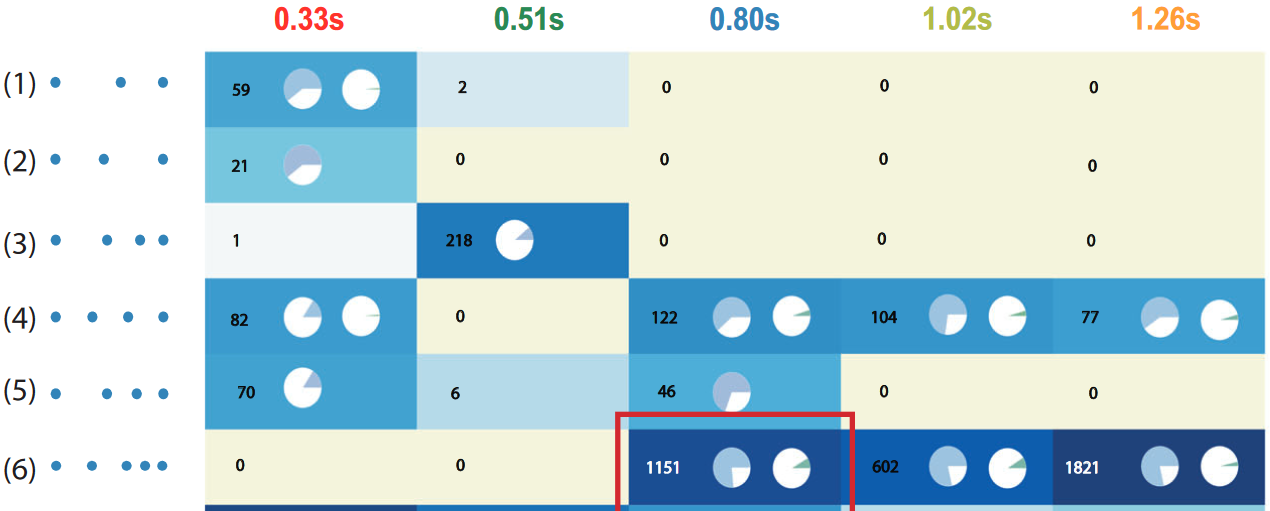
\includegraphics[width=0.5\linewidth]{images/whale.png}
%		\caption{Part of sperm whale phonetic alphabet~\citep{sharma2024contextual}.}
%		\label{fig:whale}
%	\end{subfigure}
\caption{Previous attempts of looking for phonetic alphabets in animal vocalizations.
%\KZ{Possible to stack fig (c) on top of (d) to make them look bigger?}
}
\label{fig:phones}
\end{figure*}

Several studies have identified potential fundamental units in various non-human species. \citet{hagiwara2024ispa} proposed Inter-Species Phonetic Alphabet (ISPA), a system designed to transcribe animal sounds into text.
However this system was trained on datasets from hundreds of many different species (containing marine mammal, birds, dogs, mosquito wingbeat sounds, etc.) to obtain non-human phones~(\figref{fig:masato}). This is a coarse-grained approach and overlooks differences in vocal systems and vocal modes across species.
\citet{huang2023transcribing}'s method applied human International Phonetic Alphabet (IPA) directly to transcribe Shiba Inu voices~(\figref{fig:huang}), which restricts Shiba Inu voices to a collection of human IPAs and ignores the divide between human pronounciations and dog vocals.
\citet{li2024phonetic} used HuBERT~\citep{hsu2021hubert} to obtain phonemes in Shiba Inu sounds, however, this method does not verify that similar phonemes are the same phoneme and is weakly interpretable~(\figref{fig:li}).
\citet{sharma2024contextual} obtained the sperm whale phonetic alphabet by analyzing different combinations of rhythm and tempo in sperm whale caudals~(\figref{fig:whale}). However this method only considers acoustic variations while overlooking the inter-relation between acoustics and lexical semantics in phonemic discovery.
%may be highly restricted to sperm whales or other similar marine mammals.

In this paper, we propose an iterative approach to discover phonetic inventory through simultaneously computing vocalizations and dog ``words''. The acoustically-distinguished phones and words share fine-grained lingustic similarity with 
their counterparts in human languages. Specifically,  we first collected 13,000+ YouTube videos of
Shiba Inus, Huskies and Chihuahuas, and transcribe the dog vocals therein to a large amount 
of phone sequences, similar to the approach of \citet{li2024phonetic}. Then we use an
signal energy based method to segment each phone sequences into dog barks (also known as
candidate words). At this point, we identify in total 140 distinct phones in the 
entire corpus, and these phones form the initial candidates of a canine phonetic alphabet. 
Using a modified minimal pair algorithm and by examining the contextual information of
candidate words, we iteratively narrow the phoneme set and word set down to a
steady state. In one configuation, the algorithm terminates with an alphabet of 35 phonemes
and 278 dog words. Even though the framework does not output the specific
meanings of these words, we can computationally show that each word has a stable function and
different words have specific context of use.

Our contribution can be summarized as follows:
\begin{itemize}
\item We propose an iterative phoneme discovery algorithm that produces a phoneme alphabet
for canine vocalization for the first time, by adapting from the phoneme definition for human languages;
\item The algorithm also produces a set of dog words that are comprised 
entirely of the legal phonemes in the alphabet, and each word is used in a consistent 
context;
\item As a by-product, this iterative algorithm is capable of removing most of the bad 
phones (noises) in the original transcripts, leading to a finer phone set;
\item We also conduct automatic and human evaluations that confirm the validity of the alphabet and words discovered.
\end{itemize}


